\documentclass[cn,hazy,blue,14pt,geye,normal,]{elegantnote}
\usepackage[%
	%backend=biber,%用biber后端处理bib文件, 可选的有bibtex, bibtex8, biber, 默认为biber
	%样式文件(参考文献样式文件--bbx文件,引用样式文件--cbx)使用latex编写
	%一般可以下载提供的或标准的.bbx文件和.cbx文件,放在.tex同目录下进行引用
	%支持根据本地化排版,如:
	%	biber -l zh_pinyin texfile 按拼音排序
	%	biber -l zh_stroke texfile 按笔画排序
	%style= %引用格式和文献列表格式,有相对应的.bbx和.cbx文件
	%style=nature,%方括号数值压缩形式引用,文献列表title无引号,article类无前缀"In:", "and" 用 "&" 代替
	%style=science,%圆括号数值压缩形式引用,文献列表无and, title无引号, article类无前缀
	%style=numeric,%方括号数值引用,article类前缀"In:", title有引号,默认格式
	%style=numeric-comp,%方括号数值压缩形式引用,article类前缀"In:", title有引号
	style=gb7714-2015,%国标文献引用格式2015版, 胡振震制作
	%style=trad-abbrv,%方括号数值引用,作者名缩写
	%style=trad-abbrv,
	%bibstyle=numeric,%文献列表形式:数值格式
	sorting=nyt,%文献列表排序:姓名(n),年(y),标题(t)升序,有nty, nyt, nyvt, anyt, anyvt, ynt, ydnt, none, debug, 自定义的<name>,其中ydnt是按年份降序,默认nty,
	%citestyle=numeric-comp,%引用文献形式:数值压缩形式,同时开启sortcites=true
	%sortcites=true,%引用时自动排序
	%giveninits=true,%缩写作者名,默认为false
	maxnames=3,%至多显示三个作者
	minnames=3,%至少显示三个作者
	%abbreviate=true,%缩写Editor之类,默认为true
	date=year,%只显示年份
	%url=true,%显示url,默认为true
	%doi=true,%显示doi,默认为true
	isbn=false,%不显示isbn/issn/isrn,默认为true
	%eprint=true,%对于arxiv文章有用,默认为true
	%subentry=false,%不再细分子列a,b之类,默认为false
	%hyperref=true,%使用超链接,需要配合hyperref宏包才能起作用,默认为auto,取决于是否加载hyperref宏包
	%不显示语言
	%不显示冒号
	%backref=true,%反向引用,参考文献中列出引用所在的页码,需要在第四次再编译源文件,默认为false
	]{biblatex}%用biblatex处理参考文献
%
%\renewbibmacro{in:}{\ifentrytype{article}{}{\printtext{\bibstring{in}\intitlepunct}}}%对于article类不显示"In:"
\usepackage[%
	colorlinks,%彩色超链接
	linkcolor=blue,%蓝色定理定义交叉引用等链接
	citecolor=blue,%蓝色文献引用链接
	urlcolor=OliveGreen,%橄榄绿色网址链接,颜色需要用到xcolor宏包,用dvipsnames参数
	]{hyperref}%使用超链接
%\usepackage{makeidx}%生成索引
%\makeindex
%使用biblatex处理参考文献时用
\addbibresource{seu/bib/refers.bib}%须带参考文献库文件扩展名
%
\usepackage{mathrsfs}%使用mathscr手写花体
\usepackage{fontspec}%多语言支持
\setmainfont{CMU Serif}%使用computer modern unicode字体,主要是为了显示俄文字母
\usepackage{xeCJK}%中日韩文支持
\usepackage{texnames}%显示TeX家族标识
\usepackage{metalogo}%显示XeLaTeX,XeTeX等标识
\title{\LaTeX{}中处理参考文献的三种方法总结}
\author{\href{mailto:zalois@126.com}{zalois@126.com}}
%\institute{seu}
\date{\zhtoday}
\usepackage{array}
%\setCJKmainfont[AutoFakeBold = {2.17}]{FZLanTingHeiPro_GB18030}%设置中文主字体为方正兰亭黑Pro字体
%\setCJKmainfont[AutoFakeBold = {2.17}]{Adobe Song Std L}%设置中文主字体为Adobe 宋体
\newcommand{\hei}{\CJKfontspec{Adobe Heiti Std R}}%Adobe 黑体
\newcommand{\kai}{\CJKfontspec{Adobe Kaiti Std R}}%Adobe 楷体
\newcommand{\fs}{\CJKfontspec{Adobe Fangsong Std R}}%Adobe 仿宋
\newcommand{\lei}{\CJKfontspec[ExternalLocation=/media/sdb6/TeX/fonts/cnFonts/钢笔字/]{方正徐静蕾简体.ttf}}%徐静蕾字体

\begin{document}
%生成目录开始
%\tableofcontents
%\cleardoublepage
%生成目录结束
%
%正文开始
%\section{one}
\maketitle
\section{摘要}
	``好记性不如烂笔头。''为了防止忘记再从头查找,本文总结了\LaTeX{}中处理参考文献常用的三种方法。着重总结了用Bib\LaTeX{}处理参考文献的方法。本文使用了超链接,鼠标在有颜色的部分如果变成手形,就表示此处是超链接,鼠标点击就可访问对应的资源。
\section{关键词}
	参考文献,引用,Bib\LaTeX{},\BibTeX{}
\section{处理参考文献常用的三种方法}
\LaTeX{}中处理参考文献常用如下三种方法:第三种方法最简单,但是修改起来也是最麻烦;第二种方法是传统方法,正慢慢被第一种方法替代;第一种方法出现时间稍晚些,资料不是特别多,国内研究比较深入的是胡振震,不但写了不少教程\cite{HuShidong20200726,huzhengzheng20200602},还根据国标gb7714-2015制作了格式文件\cite{HuShidong20200726}。
\subsection{方法一:用Bib\LaTeX{}处理}
笔者最推荐的方法,灵活,强大。\(2006\)年Philipp Lehman编写了Bib\LaTeX{}包\footnote{Copyright © 2006–2012 Philipp Lehman, 2012–2017 Philip Kime, Audrey Boruvka, Joseph Wright, 2018– Philip Kime and Moritz Wemheuer.},Bib\LaTeX{}包是一个更加灵活的文献处理方式,它不仅支持更多的entry type,而且支持多次加入bib文件,支持多种不同的bib内容书写格式,也支持从远程加入bib文件,支持在文档的任何位置显示参考文献的内容。比如,你可以在论文的每一章后面添加参考文献的显示,用脚注形式显示参考文献等等。从发展的眼光来看,Bib\LaTeX{}是一个比\BibTeX{}更加先进的技术,未来肯定会取代\BibTeX{}。\par
\BibTeX{}的格式控制文件有两种,一类是参考文献列表格式文件,扩展名为bbx;一类是引用格式文件,扩展名为cbx。这两种文件都是用\LaTeX{}编写的,一般也会有提供下载,也可以自己制作。Bib\LaTeX{}控制参考文献列表显示格式的方式比\BibTeX{}灵活的地方在于,它不仅用格式文件来控制显示格式,还可以通过宏包的参数来实现精细调整控制。\par
Bib\LaTeX{}有两份值得参考的文献:一份是Philip Kime等人编写的Bib\LaTeX{}手册\cite{biblatexmanual20191201},另一份是胡振震编写的《{\LaTeX}文档中文参考文献的{Bib\LaTeX}解决方案》\cite{huzhengzheng20200602}。Bib\LaTeX{}需与biber命令配合使用。\par
实现用Bib\LaTeX{}来处理参考文献,需要分成如下\textcolor{blue}{四}步:\par
\textcolor{blue}{第一步}:制作生成bib文件;\par
\textcolor{blue}{第二步}:在导言区需要加入biblatex宏包:\par
\begin{lstlisting}
\usepackage[格式控制参数]{biblatex}
\end{lstlisting}\par
bibstyle参数对应于bbx格式文件,citestyle参数对应于cbx文件。\par
style参数对应于两个同名文件,扩展名分别为bbx和cbx。
\begin{example}
	\label{example:00}
一个具体的用国标gb7714-2015文献引用格式,按姓名年份和标题升序,作者超过3个人时只显示前三个,具有超链接功能的实例如下:
\begin{lstlisting}
\usepackage[%
	%backend=biber,%用biber后端处理bib文件, 可选的有bibtex, bibtex8, biber, 默认为biber
	%样式文件(参考文献样式文件--bbx文件,引用样式文件--cbx)使用latex编写
	%一般可以下载提供的或标准的.bbx文件和.cbx文件,放在.tex同目录下进行引用
	%支持根据本地化排版,如:
	%	biber -l zh_pinyin texfile 按拼音排序
	%	biber -l zh_stroke texfile 按笔画排序
	%style= %引用格式和文献列表格式,有相对应的.bbx和.cbx文件
	%style=nature,%方括号数值压缩形式引用,文献列表title无引号,article类无前缀"In:", "and" 用 "&" 代替
	%style=science,%圆括号数值压缩形式引用,文献列表无and, title无引号, article类无前缀
	%style=numeric,%方括号数值引用,article类前缀"In:", title有引号,默认格式
	%style=numeric-comp,%方括号数值压缩形式引用,article类前缀"In:", title有引号
	style=gb7714-2015,%国标文献引用格式2015版, 胡振震制作
	%style=trad-abbrv,%方括号数值引用,作者名缩写
	%style=trad-abbrv,
	%bibstyle=numeric,%文献列表形式:数值格式
	sorting=nyt,%文献列表排序:姓名(n),年(y),标题(t)升序,有nty, nyt, nyvt, anyt, anyvt, ynt, ydnt, none, debug, 自定义的<name>,其中ydnt是按年份降序,默认nty,
	%citestyle=numeric-comp,%引用文献形式:数值压缩形式,同时开启sortcites=true
	%sortcites=true,%引用时自动排序
	%giveninits=true,%缩写作者名,默认为false
	maxnames=3,%至多显示三个作者
	minnames=3,%至少显示三个作者
	%abbreviate=true,%缩写Editor之类,默认为true
	date=year,%只显示年份
	%url=true,%显示url,默认为true
	%doi=true,%显示doi,默认为true
	isbn=false,%不显示isbn/issn/isrn,默认为true
	%eprint=true,%对于arxiv文章有用,默认为true
	%subentry=false,%不再细分子列a,b之类,默认为false
	%hyperref=true,%使用超链接,需要配合hyperref宏包才能起作用,默认为auto,取决于是否加载hyperref宏包
	%不显示语言
	%不显示冒号
	%backref=true,%反向引用,参考文献中列出引用所在的页码,需要在第四次再编译源文件,默认为false
	]{biblatex}%用biblatex处理参考文献
	%\renewbibmacro{in:}{\ifentrytype{article}{}{\printtext{\bibstring{in}\intitlepunct}}}%对于article类不显示"In:"
\usepackage[%
	colorlinks,%彩色超链接
	linkcolor=blue,%蓝色定理定义交叉引用等链接
	citecolor=blue,%蓝色文献引用链接
	urlcolor=OliveGreen,%橄榄绿色网址链接,颜色需要用到xcolor宏包,用dvipsnames参数
	]{hyperref}%使用超链接
\usepackage[dvipsnames]{xcolor}%使用68种颜色
\end{lstlisting}\par
\end{example}
\begin{example}
	\label{example:01}
去掉注释,例\ref{example:00}可简写为
\begin{lstlisting}
\usepackage[style=gb7714-2015,sorting=nyt,maxnames=3,minnames=3,date=year,isbn=false]{biblatex}
\usepackage[colorlinks,linkcolor=blue,citecolor=blue,urlcolor=OliveGreen]{hyperref}
\usepackage[dvipsnames]{xcolor}
\end{lstlisting}\par
\end{example}
\textcolor{blue}{第三步}:和第二步一样,在\textcolor{red}{导言区}指定第一步的bib文件,注意带上bib文件的扩展名。
\begin{example}
	\label{example:02}
\begin{lstlisting}
\addbibresource{seu/bib/refers.bib}%须带参考文献库文件扩展名
\end{lstlisting}\par
\end{example}
\textcolor{blue}{第四步}:在文档中需要显示参考文献的位置,加入打印参考文献列表语句:
\begin{example}
\begin{lstlisting}
\printbibliography[title=参考文献]%title为自定义,可以不带参数,用默认设置
\end{lstlisting}
\end{example}
\subsection{方法二:用\BibTeX{}处理}
\(1986\)年Oren Patashnik引入的参考文献管理程序\BibTeX{},由于不太灵活,有些参考文献排版要求难以实现,正在慢慢被新的Bib\LaTeX{}处理方法替代。\BibTeX{}本身不需要加载任何宏包(package),但编译的时候需使用bibtex程序。\par
\BibTeX{}格式控制文件是扩展名为bst的文件,一般会有提供,也可以自己制作。由于笔者更倾向于用Bib\LaTeX{}处理参考文献的方法,这里不再叙述自定义bst文件的方法。更多\BibTeX{}资料可参考\cite{胡伟2013LATEX,chikilyyongfeng2019,mittelbach2004latex}。\par
使用\BibTeX{}处理参考文献,类似的需要如下\textcolor{blue}{三}步。\par
\textcolor{blue}{第一步}:制作生成bib文件;\par
\textcolor{blue}{第二步}:指定参考文献的格式,一般在文档末尾处加入
\begin{example}
\begin{lstlisting}
\bibliographystyle{spmpsci}
\end{lstlisting}\par
\end{example}
参考文献格式有abbrv,alpha,plain,unsrt几类标准格式可供选择。
本例用的spmpsci是Springer出版集团提供的数学、物理类文章参考文献常用的列表格式,对应于spmpsci.bst文件(可由Springer官网下载得到)。\par
\textcolor{blue}{第三步}:一般是在第二步的下一行,指定第一步的bib文件:
\begin{example}
\label{example:03}
\begin{lstlisting}
\bibliography{seu/bib/refers}%这里不需要加bib文件的扩展名
\end{lstlisting}
\end{example}
\begin{note}
	关于bib文献库的制作生成,可用JabRef程序来完成,配合\TeX{}编辑器,可以比较方便地在文档中实现参考文献的引用,可以参考笔者《Jabref和Zotero使用笔记》\cite{zalois20200424}。
\end{note}
\begin{note}
	不论用Bib\LaTeX{}或\BibTeX{}处理参考文献,都需要在文中引用bib文件中的条目,如果想把所有未引用的条目也显示出来,可以用如下语句:
\begin{lstlisting}
\nocite{*}
\end{lstlisting}
\end{note}
\begin{note}
	bib文件,最好是与文档的tex源文件放在同一目录下。如果bib文件放在其它位置,需要指定bib文件的路径,如例\ref{example:02}和\ref{example:03}中所示。
\end{note}
\begin{note}
	不论用Bib\LaTeX{}或\BibTeX{}处理参考文献,可以指定多个bib文件,文件之间需要用逗号(``,'')隔开,注意Bib\LaTeX{}方式中.bib扩展名不能省略。
\end{note}
\subsection{方法三:用thebibliography环境直接处理}
简单直接,参考文献条目很少时可以用这种方法。但不推荐这种处理参考文献的方法,因为调整起来比较麻烦,还容易出错。
\begin{lstlisting}
\begin{thebibliography}{编号样本}
\bibitem[记号]{引用标志}文献条目1
\bibitem[记号]{引用标志}文献条目2
……
\end{thebibliography}
\end{lstlisting}
\section{关于编译过程}
\subsection{使用Bib\LaTeX{}处理的编译过程}
如果用\XeLaTeX{}编译,流程如下:\par
\XeLaTeX\(\to\)biber\(\to\)\XeLaTeX\par
如需要后向超链接(就是在参考文献列表中显示该参考文献在第几页被引用),则除了为biblatex宏包设置 backref选项外,还需第4遍\XeLaTeX{}编译,编译流程如下:\par
\XeLaTeX\(\to\)biber\(\to\)\XeLaTeX\(\to\)\XeLaTeX\par
整个编译流程图如下,图的制作属于registor\cite{registor20190923}。\par
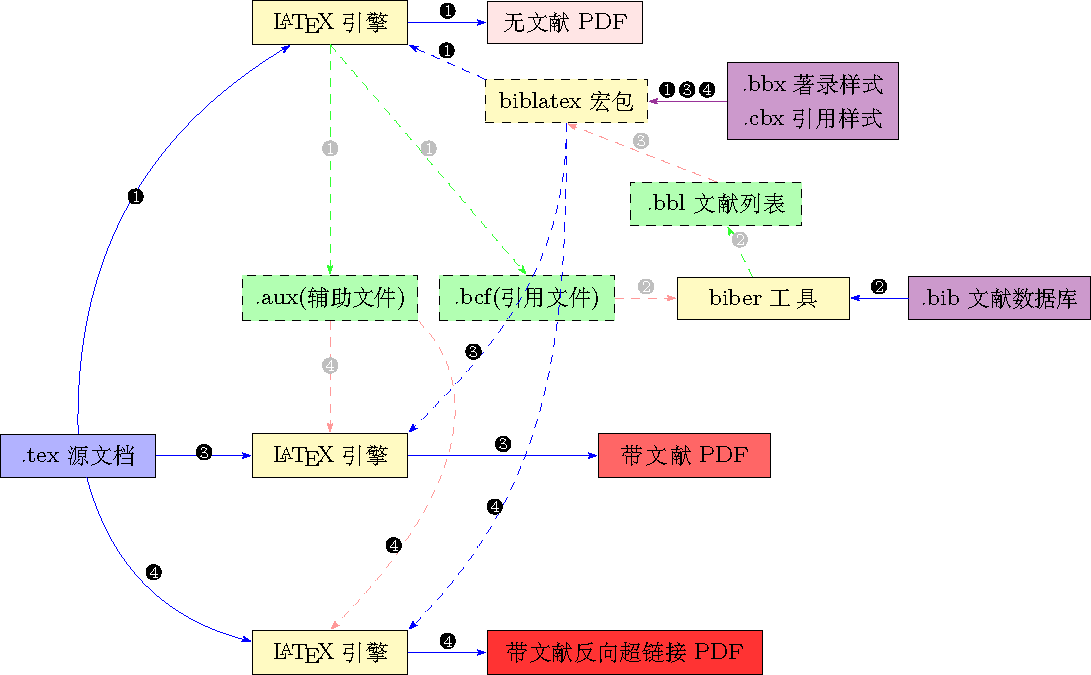
\includegraphics{BibLaTeX排版交叉引用+参考文献流程.png}
\subsection{使用\BibTeX{}处理的编译过程}
如果用\XeLaTeX{}编译,流程如下:\par
\XeLaTeX\(\to\)bibtex\(\to\)\XeLaTeX\(\to\)\XeLaTeX\par
整个编译流程图如下,图的制作属于registor\cite{registor20190923}。\par
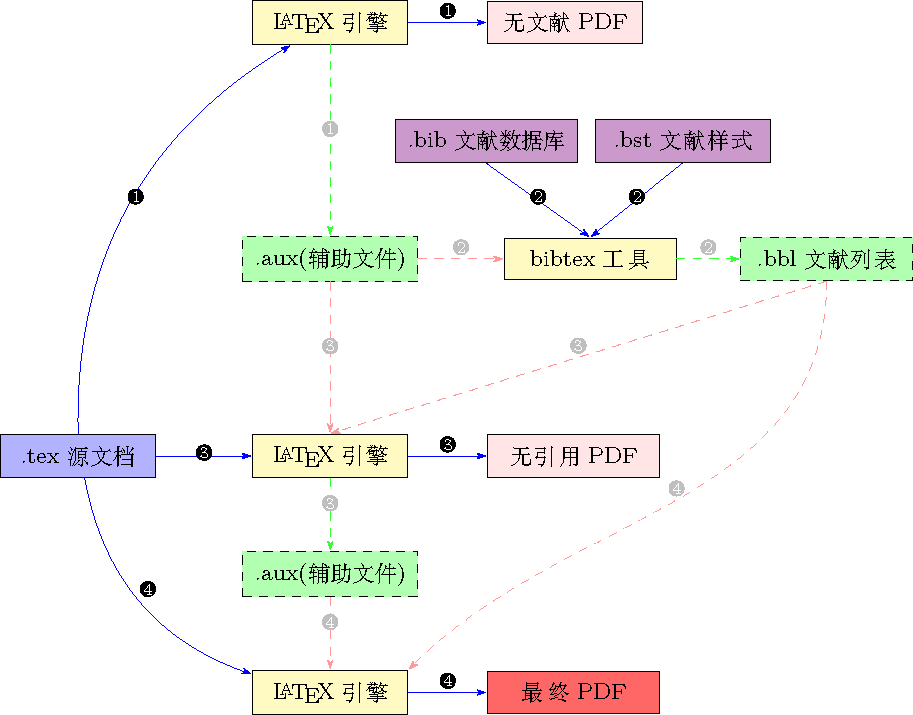
\includegraphics{BibTeX排版交叉引用+参考文献流程.png}
\subsection{使用系统提供的\LaTeX{}mk编译}
为了简化目录、交叉引用、参考文献等编译过程的自动化操作,\LaTeX{}发行版提供了``latexmk''命令,以实现一次性完成所有的编译过程,也就是用``latexmk''命令完成上述所有工作。
\begin{example}
	\begin{lstlisting}
	latexmk -xelatex jobname.tex
	\end{lstlisting}
\end{example}
\begin{example}
	\begin{lstlisting}
	latexmk -xelatex jobname.tex -c %清除临时文件,保留.bbl文件;  -C参数清除临时文件,包括pdf文件
	\end{lstlisting}
\end{example}\par
以下图给出的是\LaTeX{}常见编译过程,图片来源于网络。\par
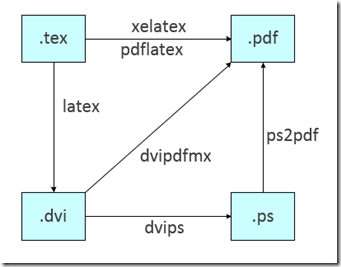
\includegraphics{LaTeX编译过程图解.png}
\nocite{*}%显示所有未引用文献
%正文结束
%
\section{利益无关声明}
本文涉及到的程序,如\TeX 系统,Jabref和Zotero文献管理器,Vim,Emacs,\TeX studio等文本编辑器都是开源软件。本文也是以开源协议发布的,欢迎大家在开源协议下自由修改分享。本文链接:\url{https://github.com/zalois/notes4references}
\section{致谢}
感谢创建\TeX 的Donald Ervin Knuth先生,感谢Jabref和Zotero的贡献者们。
本文档套用的模板下载自\href{https://github.com/ElegantLaTeX/ElegantNote}{https://github.com/Elegant\LaTeX/ElegantNote},感谢模板作者邓东升。\footnote{插播一个小广告:本文档系统环境:\href{https://mirrors.slackware.com/slackware/slackware64-current/}{Slackware64-Current} + \href{https://www.tug.org/texlive/}{\TeX live 2020} + \href{https://www.vim.org/}{Vim 8.2.1456}}
%参考文献开始
%当使用biblatex宏包时用
\printbibliography[heading=bibintoc,title=参考文献]
%在目录列表中显示参考文献
%\printbibliography[heading=bibintoc]
%
%参考文献结束
%
%生成索引页开始
%\cleardoublepage
%\phantomsection
%\addcontentsline{toc}{section}{Index}
%\printindex
%生成索引页结束
\end{document}

